%---------------------------------------------------------------
\chapter{ESP32 platform}\label{sec:esp32}
%---------------------------------------------------------------

In this chapter, a brief explanation of the ESP32 platform is presented. The main hardware and software features of the ESP32 microcontroller, which is used in this thesis, are described. The information provided is mainly based on the official ESP-IDF (the official development framework)\cite{espidf2022} and the ESP32 Technical reference manual\cite{esp322021}.

\section{Hardware}

ESP32 is a \gls{soc} microcontroller designed by Espressif which integrates CPUs, WiFi, Bluetooth and various specialized co-processors. The main features of the ESP32 are the following:

\begin{itemize}
    \item Xtensa dual-core 32-bit LX6 microprocessor running at 160 or 260 MHz
    \item 520 KB \gls{sram}, 448 KB ROM
    \item 8 KB FAST RTC \gls{sram} and 8 KB SLOW RTC \gls{sram}
    \item Wi-Fi: 802.11 b/g/n
    \item Bluetooth: v4.2 and BLE
    \item Cryptographic co-processors: RNG, RSA, SHA, AES
    \item \Gls{ulp} co-processor
\end{itemize}

One possible form factor of the ESP32 microcontroller can be seen in Figure~\ref{fig:esp32_wroom_module}. A block diagram of ESP32 functions is illustrated in Figure~\ref{fig:esp32_diagram}.

\begin{figure}[hb!]
    \centering
    \captionsetup{justification=centering,margin=0.5cm}
    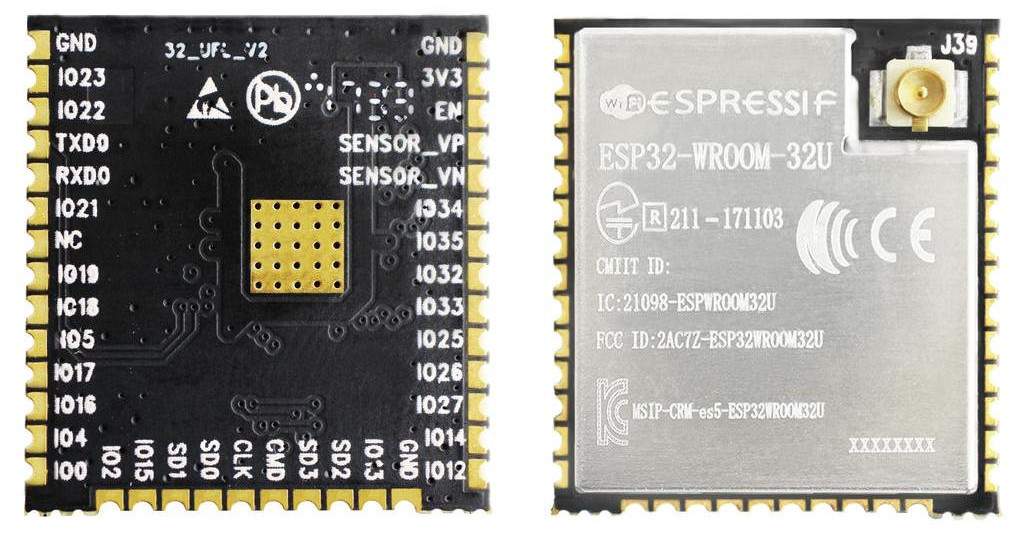
\includegraphics[width=0.45\textwidth]{images/esp32_wroom_module.jpg}
    \caption[The ESP32-WROOM-32U module back and front image.]{The ESP32-WROOM-32U module back and front image.\cite{SOSelectronic2018}}
    \label{fig:esp32_wroom_module}
\end{figure}

\begin{figure}[ht!]
    \centering
    \captionsetup{justification=centering,margin=0.5cm}
    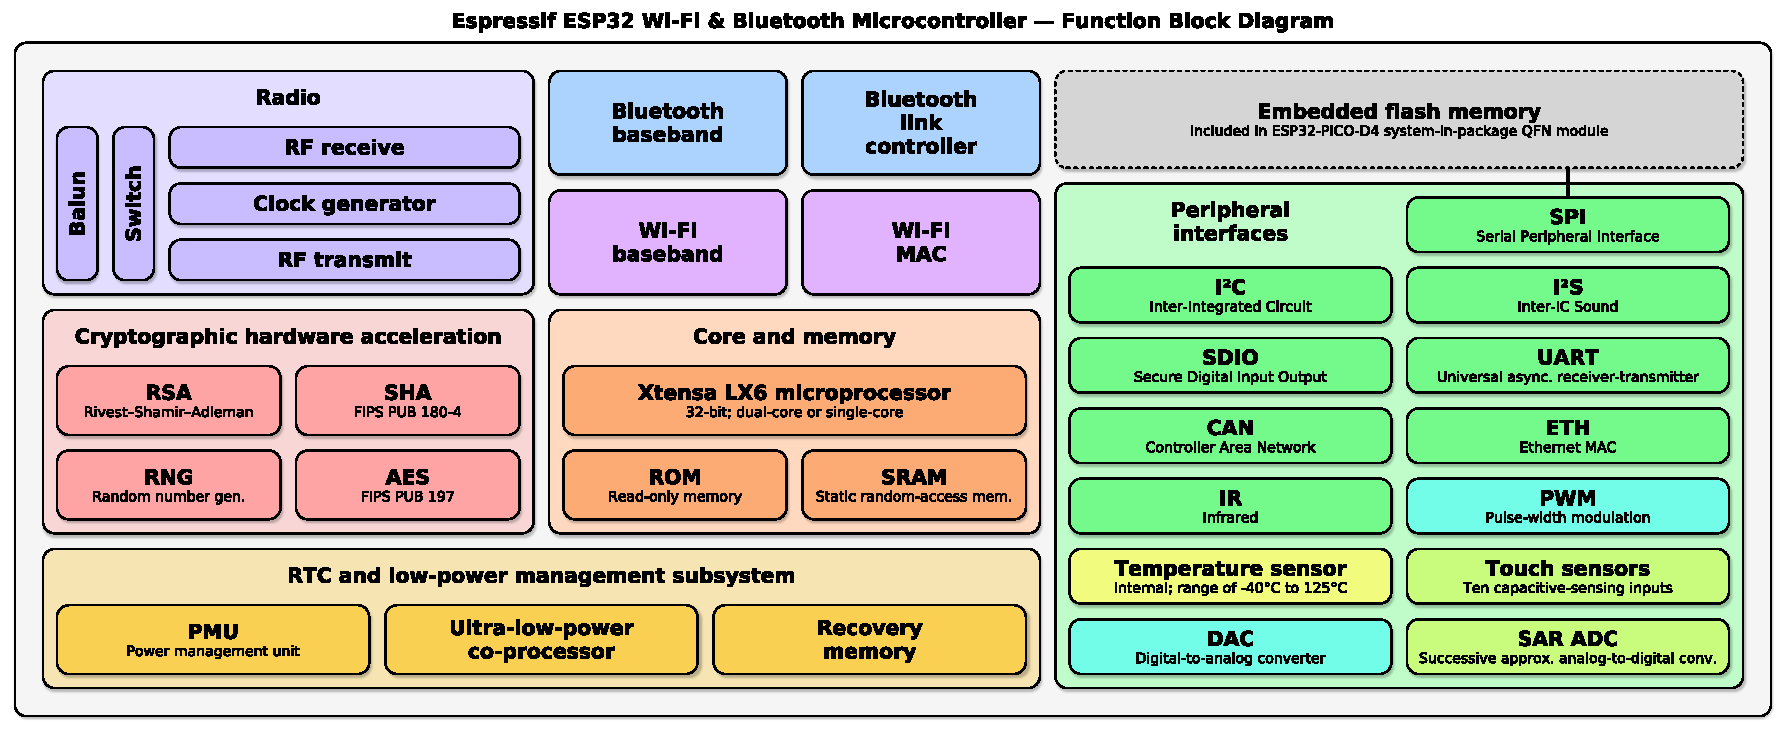
\includegraphics[width=\textwidth]{images/esp32_diagram.pdf}
    \caption[ESP32 Chip Function Block Diagram.]{ESP32 Chip Function Block Diagram.\cite{Krent2018}}
    \label{fig:esp32_diagram}
\end{figure}

ESP32 is a name for the original microcontroller from Espressif released in 2016. However, several other models have been developed since\cite{espidf2022}:

\begin{description}
    \item[ESP32-S2] A single-core version of the ESP32
    \item[ESP32-S3] Version with added instructions to accelerate machine learning
    \item[ESP32-C3] Single-core RISV-V CPU version instead of the Xtensa LX6 CPU
    \item[ESP32-S6] Single-core RISC-V CPU with WiFi 6 support
\end{description}

Only the original ESP32 microcontroller was used during experiments and implementation in this thesis. However, the possibility of implementing a \gls{sram} \gls{puf} on the other versions is discussed later in Chapter~\ref{sec:implementation}.

\section{Memory layout}\label{sec:memory_layout}

Memory layout of the ESP32 is important for a \gls{sram} \gls{puf} implementation as the exact memory region used to extract the response needs to be considered. The ESP32 has several types of embedded memories and they are discussed here briefly. A detailed description of embedded memory address mapping can be seen in Table~\ref{table:memory_mapping}. The ESP32 uses a Harvard memory architecture. This means, that instructions and data use separate memories with dedicated buses.\cite{esp322021}

\begin{description}
    \item[ROM 0 and 1] \hfill \\
        \Gls{rom} is used by the hard-coded first-stage bootloader for instructions (\gls{rom} 0) and static data (\gls{rom} 1).
    \item[SRAM 0, 1 and 2] \hfill \\
        \Gls{sram} 0 is used for program instruction. \Gls{sram} 1 is mapped to both instruction and data bus simultaneously. It can also be mapped over part of \gls{rom} 0. \Gls{sram} 2 is used for program data.
    \item[FAST RTC SRAM] The 8 KB FAST \gls{rtc} \gls{sram} is mapped to both instruction and data buses and is not turned off during power-saving modes (such as deep or light sleep). It is therefore used to keep data between the power-saving modes. Only the PRO\_CPU\footnote{The two CPU cores are named PRO\_CPU and APP\_CPU} can use this memory.
    \item[SLOW RTC SRAM] The 8 KB SLOW \gls{rtc} \gls{sram} is mapped to a region shared by both the instruction and data buses. It is clocked slower compared to the other \gls{sram} memories. It is not turned off during power-saving modes and can be used to keep data between them. The \gls{ulp} co-processor also uses it as its memory.
\end{description}

Flash memory can either be embedded inside the \gls{soc} or connected externally using \gls{spi}. A maximum of 16 MB of flash is supported and up to 8 MB of external \gls{sram} can also be connected using \gls{spi}.

\begin{table}[ht!]
    \centering
    \captionsetup{justification=centering,margin=0.5cm}
    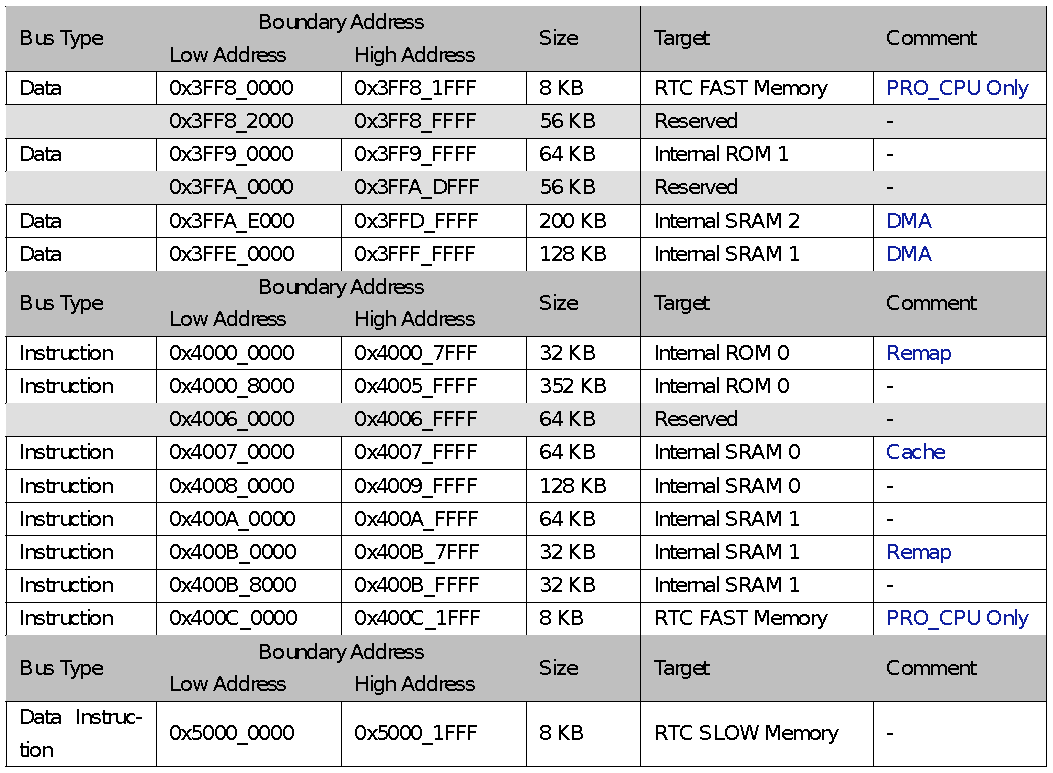
\includegraphics[width=\textwidth]{images/memory_mapping.pdf}
    \caption[ESP32 embedded memory address mapping.]{ESP32 embedded memory address mapping.\cite{esp322021}}
    \label{table:memory_mapping}
\end{table}

\section{Device startup}\label{sec:device_startup}

There are several steps involved between power-up and the start of the user application. It is important to understand them as some will be crucial to the implementation of the \gls{sram} \gls{puf}. The steps are following:

\begin{enumerate}
    \item The CPU executes the first-stage bootloader located in \gls{rom}. If the device was reset from deep sleep, a \emph{deep sleep wake stub} is executed. The second-stage bootloader is then loaded from the flash and executed.
    \item The second-stage bootloader loads the partition table from flash. The rest of the application is then loaded according to the partition table. Secure boot, over-the-air updates and flash encryption are also implemented in the second-stage bootloader.
    \item C runtime and FreeRTOS are initialized. Finally, the main task of the user application is called and the booting process is complete.
\end{enumerate}

The \emph{deep sleep wake stub} is a mechanism that enables the user to run custom code early in the boot process after waking up from deep sleep. It is implemented as a function stored in the FAST \gls{rtc} \gls{sram}. This function is then called by the first-stage bootloader before it loads the second stage.\cite{espidf2022}

\section{ESP-IDF}

ESP-IDF is an integrated development framework by Espressif. It contains libraries and source code for the ESP32 family of microcontrollers and provides a unified \gls{api} which is shared between the different microcontroller models. It also provides scripts for operating the toolchain, uploading applications and monitoring them.\cite{espidf2022}

The latest stable version of ESP-IDF (on \today) is 4.4 and this version was used for all code used in this thesis on the ESP32 microcontrollers.

\begin{figure}[h!]
    \centering
    \captionsetup{justification=centering,margin=0.5cm}
    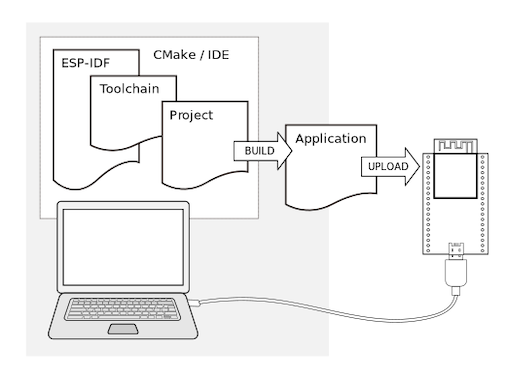
\includegraphics[width=0.45\textwidth]{images/upload_process.png}
    \caption[Development of applications for ESP32]{Development of applications for ESP32.\cite{espidf2022}}
    \label{fig:upload_process}
\end{figure}

\section{FreeRTOS}

A modified version of the \gls{rtos} FreeRTOS is used in ESP-IDF to create applications. Its main feature is enabling symmetric multiprocessing in order to utilize both CPU cores. Tasks play the role of threads and Wifi, Bluetooth and user tasks can be created and are managed by a real-time scheduler. The FreeRTOS also provides inter-task communication and synchronization \gls{api}.\cite{espidf2022}
